\chapter{Capture and Replay for Eiffel}
\eiffellisting
\section{Differences to Existing Implementation}
Selective capture and replay as described by Joshi and Orso \cite{orso05may} can not be directly applied to Eiffel. Although the core elements of the technique can be used in Eiffel, too, we need to adapt some parts. In this section the changes to the original implementation and reasons for these changes will be discussed.

\subsection{Language Aspects}
Even though Java and Eiffel are both object oriented languages, there are differences between these two languages, syntax left aside. Eiffel offers a wider set of language constructs, many times trying to solve problems inherently object oriented, whereas Java reused solutions from its ancestors, mainly C++. One example for this difference could be the Eiffel basic types, which can be treated as objects with methods and attributes versus the Java basic types, which are no objects. This section focuses on the differences between Java and Eiffel that influenced our implementation of selective capture and replay.

\subsubsection{Terminology} % diesen Titel weglassen?
Eiffel has a nomenclature that differs from other programming languages. Here the Eiffel terminology is described according to \cite{oosc2} and compared to the one from Java.
\begin{center}
\begin{tabular}[]{|l|l|} \hline
 \textbf{Eiffel}&\textbf{Java} \\ \hline
 Attribute&Field \\ \hline
 Ouery&Field or Method that has a return value \\ \hline
 Routine&Method \\ \hline
 Procedure&Method that has no return value \\ \hline
 Function&Method that has a return value \\ \hline
 Feature&Method or Attribute \\ \hline
 ANY&Object (ancestor of all classes) \\ \hline
\end{tabular} 
\end{center}

\subsubsection{Multiple Inheritance}
Eiffel is designed to support multiple inheritance, whereas in Java, only single inheritance is allowed. The original implementation assumes, that all subclasses of a class \emph{c} are in the observed set iff \emph{c} is also in the observed set. This makes it possible to statically decide whether an observed or an unobserved feature is accessed.

If this assumption is translated to multiple inheritance, it would not be possible to have a class \emph{C} that inherits both from an observed class \emph{A} and an unobserved class \emph{B} (\figref{fig:obs_unobs_multiple_inheritance}).
\begin{figure}[ht]
  \centering
  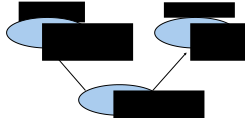
\includegraphics[width=0.5\textwidth]{illustrations/obs_unobs_multiple_inheritance}
  \caption{Conflict Due to Multiple Inheritance}
  \label{fig:obs_unobs_multiple_inheritance}
%\includegraphics{illustrations/capture_and_replay_generic_structure}
\end{figure}

Multiple inheritance is extensively used in Eiffel, thus this assumption would be too restrictive in our opinion. It would lead to big clusters that could not be divided into observed and unobserved set. 

Although Java does not allow multiple inheritance, it supports multiple interface inheritance. Joshi and Orso \cite{orso05may} mention that they need to dynamically determine if the target of an event is observed or unobserved in certain cases. We assume that multiple interface inheritance with a class that both implements an observed and unobserved interface  is at least one of these cases. They use the \texttt{instanceof} operator determine if an object is an instance of an observed class.

We will present a solution that always determines dynamically, if an object is an instance of an observed class (\emph{observed object}) or an instance of an unobserved class (\emph{unobserved object}), together with a proposal how to solve this problem without reflection.

\subsubsection{Read Only Attributes}
Eiffel strictly follows the \emph{uniform access principle} \cite{oosc2}. The principle states that it should not be visible to the clients whether features are implemented through storage or computation. This ensures that the implementation of a feature could be changed from attribute to function or vice versa. One of the consequences of this principle is that clients of a class cannot write to attributes, as these attributes could be implemented as a function as well.

In Java, this principle is not ensured because clients of a class can write to their fields. For our implementation of selective capture and replay, this limits the events related to field accesses to OUTREAD. Both OUTWRITE and INWRITE can not happen, because write access to fields is restricted to their class, thus there can not be any write accesses to fields from observed to unobserved classes or reverse.

\subsection{Target Application}
As a first application that could use selective capture and replay in Eiffel, Cdd, a tool for Contract Driven Development \cite{cdd07} was chosen. Cdd allows programmers to extract test cases from failing program runs. The contracts that are present in the code are used as test oracles.Cdd is not always able to generate such a test case, due to different reasons:

\begin{description}
\item [Prestate extraction:] The state before calling the failing feature (which is needed to generate a test case) is extracted using the state at the time of failure. Because not all instructions between feature call and failure can be undone, the extraction of the prestate is not always possible.
\item [Non-determinism:] If the failing feature reads values from sources that don't always return the same values (eg. user input), it's not generally possible to run the test cases with the same result as in the failing run.
\item [External state:] When the feature relies on state that is not stored in Eiffel objects (e.g. in C structs), Cdd is not able to gather this state for the test.
\end{description}

All these limitations can be resolved using selective capture and replay:
\begin{description}
\item [Prestate extraction:] By setting a breakpoint at the beginning of the failing feature, it is possible to extract the prestate during the replay of the application.
\item [Non-determinism:] When adding all non-deterministic classes to the unobserved set, it can be ensured that the replay of the run is deterministic.
\item [External State:] All classes that wrap external state can be added to the unobserved set. Thus interactions with these classes can be replayed without having to store the external state.
\end{description}

Prestate extraction using selective capture and replay requires an immediate rerun of the application under test. Because complete recompiles in Eiffel last for tens of minutes up to hours, we can not afford to instrument the application again before replaying it. Thus it is necessary to design the code instrumentation to be both applicable for capture and replay phase. We pushed this approach even further to allow the user to disable the whole instrumentation. This allows execution with minimal overhead if capture and replay is not needed without recompiling the application.

\section{Code Instrumentation}
\subsection{Outline}
Due to differences between Eiffel and Java and a different use case, there are two main differences between the original implementation and our approach:

\begin{enumerate}
 \item It is necessary to determine dynamically whether an object is observed or not.
\item It must be possible to switch between capture and replay phase without reinstrumenting the code.
\end{enumerate}

The first requirement can be met by adding an additional query to every class so that it is possible to find out whether an object is an instance of an observed or an unobserved class. We ensure that every class has this query by adding it to ANY. In the next chapter we will discuss how this query can be implemented efficiently.

In order to be able to switch between capture and replay mode, the class PROGRAM\_FLOW\_SINK was introduced. Program flow events are put into the PROGRAM\_FLOW\_SINK. It is both the ancestor class of RECORDER, the class that contains the management code for recording events and PLAYER, the class that provides the scaffolding for replaying events. The standard instance of a PROGRAM\_FLOW\_SINK is globally accessible. It is dynamically bound to an instance of RECORDER during capture phase and PLAYER during replay phase.

To create placeholder objects from unobserved classes, their original routine bodies are disabled during replay pha phase. When replaying, the routines only execute instrumentation code that invokes the scaffolding and takes care of the return value if necessary.

\subsection{Routines}
Whereas the original implementation captures routine calls by instrumenting the call site (in the client), we decided to instrument the calee (the supplier). This simplifies code instrumentation, because there is no need to make changes inside existing routine bodies, it is sufficient to add some code at the beginning and the end of the routine bodies. %TODO Gibt es noch ein besseres Motiv?

The routine instrumentation can be divided into three parts (\figref{fig:routine_instrumentation_structure}): Right at the beginning of the routine, code to detect call events is inserted. The original routine body is made conditional so that it is not executed for unobserved routines during the replay phase. Finally, code to detect callret events is inserted at the end of the routine.
\begin{figure}[ht]
  \centering
  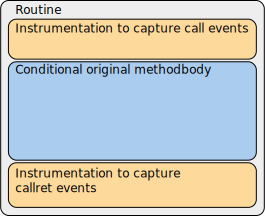
\includegraphics[width=0.5\textwidth]{illustrations/routine_instrumentation_structure}
  \caption{Structure of Routine Instrumentations}
  \label{fig:routine_instrumentation_structure}
\end{figure}

To explain instrumentation in more detail, we describe each of these three parts using the command \texttt{withdraw} of the class \texttt{ATM} (\listref{lst:account_exists_original}).

\begin{lstlisting}[caption=Original Code of Command \texttt{withdraw} ,label=lst:account_exists_original]
account_exists (account_name:STRING): BOOLEAN
		-- Is there an account with name 'account_name'?
	require
			account_name_not_void: account_name /= Void
	do
		Result := (the_bank.account_for_name (account_name) /= Void)
	end
\end{lstlisting}

\subsubsection{Capturing Call Events}
To capture call events, instrumented code, which is only executed when capture and replay is enabled, is inserted at the beginning of every routine. The code first detects whether the routine was called across the boundaries. If that is the case, it puts the associated event into the program flow \listref{lst:invocation_instrumentation}
\begin{lstlisting}[caption=Instrumentation Code to Detect Call Events,label=lst:invocation_instrumentation]
if program_flow_sink.is_capture_replay_enabled then
	program_flow_sink.enter
	if program_flow_sink.observed_stack_item /= is_observed then
		program_flow_sink.put_to_observed_stack (is_observed)
		program_flow_sink.put_feature_invocation ("account_exists", Current, [account_name])
	else
		program_flow_sink.put_to_observed_stack (is_observed)
	end
	program_flow_sink.leave
end
\end{lstlisting}
Note that all the inserted code is part of the selective capture and replay management code, which does not belong to the code of the original application. Thus these instructions must not trigger further events for the event log (e.g. the creation of the manifest string ``withdraw'' should not create other call events on class STRING). To make sure, that this won't happen, the commands \texttt{enter} to disable capture and replay and \texttt{leave} to reenable capture and replay were implemented.

To detect boundary crossing calls, the management code keeps an own stack that indicates whether the target objects of the calls on the call stack are observed or not. This stack is managed in parallel to the call stack; in the invocation instrumentation code, the result of the query \texttt{is\_observed} is put onto the stack and in the exit instrumentation code, thes value is removed again. Using this stack, it is possible to find out, whether the caller object was observed or not.
\subsubsection{Conditional Routine Body Execution}
To be able to switch between the original and the placeholder routine body, the original routine of unobserved routines is only executed during capture phase. Placeholder routines are only needed for unobserved routines, thus the original body is always executed for observed routines (\listref{lst:methodbody_instrumentation}). The query \texttt{is\_replay\_phase} always returns false, when capture and replay is disabled, therefore the management code will always use the original routine body.

\begin{lstlisting}[caption=Conditional Methodbody,label=lst:methodbody_instrumentation]
if (not program_flow_sink.is_replay_phase) or is_observed then
	Result := (the_bank.account_for_name (account_name) /= Void)
end
\end{lstlisting}
\subsubsection{Capturing Callret Events}
To capture and replay callret events, instrumentation code is inserted at the end of the routines. Again, the code only puts an event into the \texttt{program\_flow\_sink} if the routine was called across the boundary. If the routine is a function, the code also restores the result that was computed in the capture phase for unobserved functions. The result is only restored for unobserved classes during replay phase, otherwise the query \texttt{last\_result} returns the same value that was put into the \texttt{program\_flow\_sink} before. Thus functions can be used as placeholder functions without altering the instrumentation between capture and replay phase.
\begin{lstlisting}[caption=Instrumentation to Capture Callret Events,label=lst:exit_instrumentation]
if program_flow_sink.is_capture_replay_enabled then
	program_flow_sink.enter
	program_flow_sink.remove_from_observed_stack
	if program_flow_sink.observed_stack_item /= is_observed then
		program_flow_sink.put_feature_exit (Result)
		Result ?= program_flow_sink.last_result
	end
	program_flow_sink.leave
end
\end{lstlisting}

\subsubsection{Complete Routine Instrumentation}
\listref{lst:account_exists_instrumented} shows the routine after combining all three parts of the instrumentation.
\begin{lstlisting}[caption=Routine \texttt{account\_exists} After Instrumentation,label=lst:account_exists_instrumented]
account_exists (account_name: STRING_8): BOOLEAN
		-- Is there an account with name 'account_name'?
	require
		account_name_not_void: account_name /= Void
	do
		if program_flow_sink.is_capture_replay_enabled then
			program_flow_sink.enter
			if program_flow_sink.observed_stack_item /= is_observed then
				program_flow_sink.put_to_observed_stack (is_observed)
				program_flow_sink.put_feature_invocation ("account_exists", Current, [account_name])
			else
				program_flow_sink.put_to_observed_stack (is_observed)
			end
			program_flow_sink.leave
		end
		if (not program_flow_sink.is_replay_phase) or is_observed then
			Result := (the_bank.account_for_name (account_name) /= Void)
		end
		if program_flow_sink.is_capture_replay_enabled then
			program_flow_sink.enter
			program_flow_sink.remove_from_observed_stack
			if program_flow_sink.observed_stack_item /= is_observed then
				program_flow_sink.put_feature_exit (Result)
				Result ?= program_flow_sink.last_result
			end
			program_flow_sink.leave
		end
	end
\end{lstlisting}

\subsection{Attribute Accesses}
Automated code instrumentation for attribute accesses could not be implemented as part of this thesis, because the part of the Eiffel compiler code that was intended to be used for instrumentation turned out to be unsuitable for the task. Emmanuel Stapf of Eiffel Software Inc. advised us to use the mechanism that generates wrapper code for attribute accesses to support expanded generic derivation reattachment (related to autoboxing). Unfortunately the compiler could not apply the mechanism to all attribute accesses and it was not possible to make the necessary changes in the compiler due to a lack of time.

Here is a sketch how the instrumentation code for an access to \texttt{atm.ui} could look like:
\begin{lstlisting}[caption=Instrumentation of an Attribute Access]
 if program_flow_sink.is_capture_replay_enabled  and then is_observed and then (not atm.is_observed) then
	program_flow_sink.enter
	program_flow_sink.put_attribute_access("ui",atm, atm.ui)
	program_flow_sink.leave
 end
 ui := atm.ui
\end{lstlisting}
Again, the instrumentation code could be used for both capture and replay phase. The condition makes sure, that only OUTREAD events are captured and replayed. During capture phase, the \texttt{RECORDER} would log the corresponding OUTREAD event and during replay phase, the \texttt{PLAYER} would ensure that value of the attribute read in the next statement corresponds to the value that was read during capture phase. It could do so by setting the attribute to the value from the log.

The whole instrumentation needs to be put into a function that is accessed instead of the attribute, because the attribute could be accessed as part of a more complex expression:
\begin{lstlisting}
 a := other.function + other.attribute
\end{lstlisting}
It does not suffice to execute the instrumentation for the access to \texttt{other.attribute} before the evaluation of the expression, because \texttt{other.function} could have a side effect that changes \texttt{other.attribute}; although this would violate the \emph{Command-Query Separation Principle} \cite{oosc2}, it can not forbidden.

\subsection{Attribute Manipulation from C Level}
One assumption of the original selective capture and replay implementation is that native code never manipulates observed fields. Eiffel allows integration of C code into classes, using the \texttt{external} keyword. In order to write to fields of Eiffel objects, the C code needs the adress of that object, which can be done using the \texttt{\$} - operator.

To find out the classes whose fields are written from native code, we searched for the \texttt{\$} operator in the Eiffel base library. Only writes to \texttt{{STRING}.area} of type \texttt{SPECIAL [CHARACTER]} were identified to cause problems. Other than that, there were some write accesses to fields of the class that contain the C code, which is unproblematic because these accesses can cross the boundaries.
Restricting the class \texttt{STRING} to be in the unobserved set was not an option, because it would imply serious performance penalties to applications that havily use strings (e.g. a parser). To address this issue in a different way, the command \texttt{note\_direct\_manipulation} was added to the class \texttt{SPECIAL}, which needs to be called whenever unobserved C code writes to the fields of \texttt{SPECIAL}. Due to the lack of other use cases, the command was only implemented to support \texttt{SPECIAL [CHARACTER]}. During the capture phase it writes down the new content of the object and when replaying the corresponding event, that content is restored, thus the objects are in the same state during replay as the were in the capture phase.

Manifest strings are another case where C code writes to strings, because the C code generated by Eiffel Studio allocates and initializes these strings directly. No automated instrumentation for manifest strings was implemented, but it could be added by modifying the C macro that is used to generate manifest strings.

\section{Architecture}
In this chapter, we will explain the architecture of the management code. \figref{fig:implementation_overall_architecture} shows the key classes of the implementation with the \texttt{PROGRAM\_FLOW\_SINK} as the entrance point to the management code. Program flow events are put into the standard instance of it, which all classes can access through the once function \texttt{\{ANY\}.program\_flow\_sink}; during capture phase, it is set to an object of type \texttt{RECORDER} and during replay phase, it is set to an instance of \texttt{PLAYER}.

\texttt{RECORDER} uses \texttt{SERIALIZER} to write events to a log file.
\begin{figure}[ht]
  \centering
  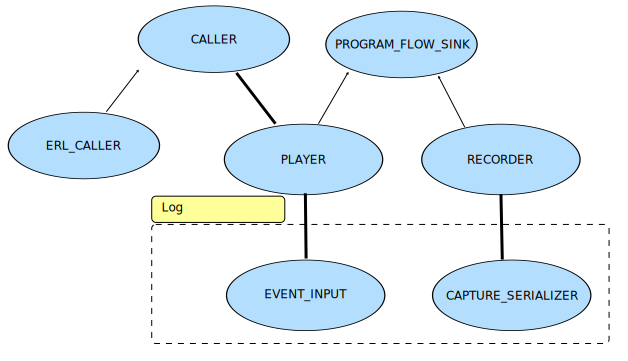
\includegraphics[width=0.8\textwidth]{illustrations/implementation_overall_architecture}
  \caption{Overall Architecture of the Implementation}
  \label{fig:implementation_overall_architecture}
\end{figure}
\subsection{The Event Log}
First it was intended to use XML as the Format for the log files because there would be no need to write a parser end the format could be verified using XSD. For our parser, it was required to parse one event at a time, because the log files can become quite big. With the Gobo XML parser, it's not possible to request parsing of one XML element at a time, there are only the options to use event based parsing or DOM parsing. Using the event based parser was mandatory, because the DOM based parser would eat up to much memory with big log files. The event based mode did not fit, because this required to invoke the replay harnest from the parser and not vice versa. It would have been possible to put the parser into an own thread and block this thread whenever one element is buffered and not yet consumed by the replay harnest. Multithreading in eiffel requires a compiler switch which causes alternative, incompatible libraries to be used. Thus this was not an option, because it would render the capture/replay mechanism unusable for single threaded applications.
Because of these limitations in XML, the event log is written to a line based textfile, whose format is defined in the grammar from (\ref{lbl:log_file_grammar}).

The classes related to the log were designed to allow addition of other log formats in the future. For example \texttt{RECORDER} is using the deferred class \texttt{CAPTURE\_SERIALIZER}, whose descendants can use their own log format (\figref{fig:implementation_serializer}). The deferred class offers a command for each event type to write the corresponding event to the log (e.g. \texttt{write\_incall}) and \texttt{TEXT\_SERIALIZER} implements these commands by writing out the events according to the grammar.

\begin{figure}[ht]
  \centering
  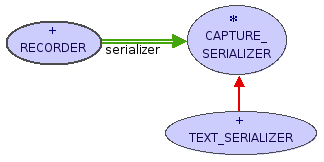
\includegraphics[width=0.5\textwidth]{illustrations/implementation_serializer.png}
  \caption{\texttt{CAPTURE\_SERIALIZER} and \texttt{TEXT\_SERIALIZER}}
  \label{fig:implementation_serializer}
\end{figure}

The parser is divided into the class \texttt{EVENT\_PARSER} that reads from the log and \texttt{EVENT\_PARSER\_HANDLER} to handle events that were generated by the parser (\figref{fig:implementation_parser}). \texttt{\{EVENT\_PARSER\}.parse\_event} parses the next event from the log and calls the apropriate handler from \texttt{EVENT\_PARSER\_HANDLER} afterwards, for example \texttt{handle\_incall\_event}.  
\texttt{TEXT\_EVENT\_PARSER} is a recursive descent parser \cite{aho86} that parses the line based log file. To support other log formats, it is possible to implement other parsers that inherit from \texttt{EVENT\_PARSER}.
The player reads events from the class \texttt{EVENT\_INPUT}, which uses the parser to read the events from the log.

%Typ des Parsers
\begin{figure}[ht]
  \centering
  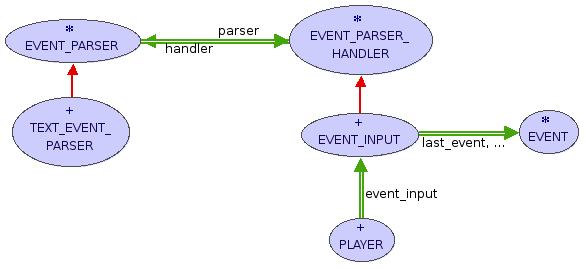
\includegraphics[width=1\textwidth]{illustrations/implementation_parser.png}
  \caption{Architecture of the parser}
  \label{fig:implementation_parser}
\end{figure}

\subsection{The Recorder}
The recorder receives the events that were passed to the program flow sink and records them to the log. To determine whether a call is an incall or outcall, it uses the \texttt{is\_observed\_stack} that indicates for all routines on the call stack whether they are observed or not. Then, the recorder writes the event to the log, using the \texttt{CAPTURE\_SERIALIZER}.
\subsection{The Player}
%Wann werden die Events konsumiert?
%Wie werden die Events konsumiert?
%Welches ist jeweils der letzte Event des Event Inputs?
%entity resolver
%Caller
%Simulate unobserved body...
%detektieren von out of sync events
%Registrieren der Object - Id's
%Play
%unterschiedliche Parts noch genauer beschreiben
\section{Advantages over Traditional Capture and Replay}
\section{Limitations}
%unter welchen Umstaenden musste manuell instrumentiert werden??
\section{Future Steps}
%Fehlende features + idee zu deren implementierung

\section{Building the Example from Source}
In this section the process of building an example with capture replay support under Linux will be described. Setting up the modified version of Eiffel Studio and all necessary tools will take the biggest part of this explanation.\\
%TODO: wieso genau wird eine modifizierte Version von Eiffel Studio benoetigt??
It is assumed that all commands in the following steps are executed in the same session, thus keeping the environment variables.\\

\subsection{Building the Preliminaries}
The first tools we need are the  Eiffel Studio Tools \cite{estudiotools}. These will be used in many setup scripts in the examples or tests from the repository. Install those tools according to the description on the webpage.\\

The delivery of the modified Eiffel Studio was built using revision 69201 of Eiffel Studio. Building a delivery with a later version of Eiffel Studio was not testet, so it might not work. If no binaries of revision 69201 are available, a delivery of that revision from source \texttt{(stimmt das wirklich??? gaebe das kein Henne / Ei Problem?)}.\\
After copying the delivery to ~/estudio/Eiffel60\_gpl\_69201, it can be activated:
\bashlisting
\begin{lstlisting}
   activate_estudio 60_gpl_69201
\end{lstlisting}

Now Gobo \cite{gobo} can be installed can be installed from svn (Revision 6001 was successfully tested).
- Install Gobo  from svn (revision 6001) -->
\begin{lstlisting}
svn co -r6001 https://gobo-eiffel.svn.sourceforge.net/svnroot/gobo-eiffel/gobo/trunk ~/capture_replay/gobo
export GOBO=~/capture\_replay/gobo
export PATH=$GOBO/bin:$PATH
$GOBO/work/bootstrap/bootstrap.sh gcc ise
\end{lstlisting}

As all preliminaries are installed, Erl-G \cite{erlg} can be downloaded and built. Revision 719 of Erl-G was tested together with capture and replay.
\begin{lstlisting}
svn co -r719 https://svn.origo.ethz.ch/autotest/trunk/erl_g ~/capture_replay/erl_g
export ERL_G=~/capture_replay/erl_g
export PATH=$ERL_G/bin:$PATH
cd $ERL_G
#EIFFEL_SRC is needed. avoid conflicts between EIFFEL_SRC and ISE_LIBRARY.
export ISE_LIBRARY=$EIFFEL_SRC
geant install
geant compile
\title{Selective Capture and Replay for Eiffel
\end{lstlisting}

To build a delivery of the modified Eiffel Studio, execute these commands: (this will take a few hours).
\begin{lstlisting}
cd ~/capture_replay/
mkdir es
svn co https://eiffelsoftware.origo.ethz.ch/svn/es/branches/capture_replay es
export EIFFEL_SRC=~/capture_replay/es/Src
cd es
geant -b $EIFFEL_SRC/scripts/build.eant build_es
\end{lstlisting}

Before an example can be built the delivery that was just created needs to used be set as default instance of Eiffel Studio
\begin{lstlisting}
cd ~/estudio
ln -s ~/capture_replay/es/EiffelXX EiffelCR
activate_estudio CR
\end{lstlisting}

In order to make the created Eiffel Studio use a modified version of the runtime, it is necessary to recompile the runtime with modified CFLAGS. The new version of the runtime then needs to be installed in the delivery.

It is not possible to directly build Eiffel Studio with the modified version of the runtime, because the changes in the runtime are not compatible to Eiffels store mechanism (\texttt{TODO: das auch noch unter irgendwelchem future work anmerken...}). This would render Eiffel Studio unusable because it relies on this mechanism during the build process.
\begin{lstlisting}
export CFLAGS='-DCAPTURE_REPLAY' 
cd $EIFFEL_SRC
#build the runtime from scratch (clobber the old one)
geant -b scripts/build.eant compile_runtime
cd $ISE_EIFFEL/studio/spec/linux-x86/lib
rm *
cp $EIFFEL_SRC/C/run-time/lib* .
\end{lstlisting}


\subsection{Building an Example}
Now, all necessary tools should be installed and the corresponding environment variables set. And we can start to build an example.\\
First we need to add reflection support to the example project. Erl G will generate reflection classes for us. If the environment variables are correctly set, the geant script should invoke Erl G automatically. \\
At the moment Erl-G does not support overrides because this feature is missing in the Gobo parser. Therefore it's necessary to override the necessary classes manually. There are two geant tasks that take care of this:

\begin{itemize}
\item \identifier{patch\_elks} makes the manual override by copying the modified elks classes from \$EIFFEL\_SRC/library/base/capture\_replay/elks\_overrides to \$ISE\_LIBRARY/library/base/elks \\
\item \identifier{unpatch\_elks} restores the original state by copying the original elks classes from \$EIFFEL\_SRC/library/base/elks to \$ISE\_LIBRARY/library/base/elks .
\end{itemize}

\begin{lstlisting}
cd ~/capture_replay/es/examples/capture_replay/iteration1
geant install
\end{lstlisting}

The example can now be opened with the modified version of Eiffel Studio. Make sure that the CFLAGS are still set to '-DCAPTURE\_REPLAY'. Otherwise it will not be possible to build the example.



\section {Limitations}
%-Konstruktoren nach ANY exportiert (fehlende unterstuetzung von Eiffel-Seite fuer Konstruktoren)
%- Access modifiers e.g. export of a observed feature only to an unobserved class --> replay not possible.